\section{Cluster-based Map Abstraction}
\label{aha:mapabstraction}
The annotated graph we have focused on creating to now is sufficient for computing a low-level strategy but inefficient for large problem sizes. 
Instead of planning every step, we would prefer to express a more general strategy using macro-operations.
We will achieve this by extending the off-line decomposition technique described in \cite{botea04} to deal with large agents and multiple terrains. Their general process involves dividing a grid map into \emph{clusters} and \emph{entrances}. 
\begin{definition}
A \emph{cluster} is a subset of the original grid map which results when the map is divided into a set of adjacent sections. 
\end{definition}

\begin{definition}
An \emph{entrance} is a contiguous area (ie. obstacle free) between two adjacent lines of tiles $l1$ and $l2$ that represent the border of clusters $c1$ and $c2$. 
Each entrance is associated with a particular \emph{size} (the length of the maximally sized contiguous area) and \emph{orientation} (either veritcal or horizontal depending on the nature of the adjacency). If obstacles exist along the border between two clusters, several entrances may be created.
\end{definition}

In figure \ref{aha-fig:abstractgraph}(a) We show the result of a simple division using a fixed-size square cluster approach. In this case, our toy map is divided into 4 adjacent clusters. \\ \newline
Building entrances is likewise straightforward. We must scan the border of every cluster where it is adjacent to another in order to determine if one is reachable from the other. In the original work, once an entrance is identified, transitions are created between the clusters by adding a pair of connected nodes to the abstract graph which represent key locations along the entrance area. In our case, we choose as the transition point the pair of nodes which maximise the clearance value for a given capability. We compute this latter metric by taking the minimum clearance among each node pair in the entrance area and selecting the largest value from the resultant set. \\ \newline
We proceed in this way and scan the entrance area for transitions for each available capability. When a maximally sized transition is located, we annotate the resultant abstract edge with the newly discovered clearance value and the capability used to find it. \\
We do not need to add any annotations to our abstract nodes; it is sufficient to define the length and traversal requirements of the corridor connecting them.  

\begin{definition}
A \emph{corridor} is a set of connected traversable nodes in the grid environment which connect a pair of locations. The length of a corridor is the sum of the traversal costs of all the nodes in the corridor set. A corridor is associated with a particular capability which must include the terrain type of every node in the corridor set. 
The width of a corridor is the minimum clearance value for some given capability among all nodes in the corridor set. 
\end{definition}

Figure \ref{aha-fig:abstractgraph}(b) highlights our decomposition process. On the left we present two adjacent clusters, while on the right are the three entrances identified and their respective transition points. \emph{E1} and {E2} are discovered using single-terrain capabilities, while \emph{E3}, which spans the whole border area, is discovered using a more complex multi-terrain capability. 
Note that \emph{E3} shares the same the location on the low-level map with \emph{E1} since we actively attempt to re-use any existing abstract nodes in case multiple transitions are identified at the same location in the original grid map. If the existing abstract nodes are already connected we also attempt to re-use the edge between them by checking if the existing edge is traversable using the capability and maximal clearance values of the proposed transition. In our example \emph{E3} represents a wider corridor than \emph{E1} so we add a new edge to the abstract multi-graph. \\
\medskip
Our final step to complete the abstraction involves connecting each abstract node to every other reachable abstract node in the local cluster. 
We achieve this by using AA* to search for the optimal path between each pair of nodes for all available capabilities and agent sizes. 
Once a path is found we insert a new undirected edge into the abstract graph to connect the two nodes using the path distance as its cost and annotating it with the capability and clearance parameters used by AA* to find the solution. 
To avoid edge duplication when pathfinding inside each  cluster we will order from lagest to smallest the set of available agent sizes which we pass as clearance parameters to AA*. 
We also order the capability parameters we pass to AA* from simplest (those containing the least number of terrains) to most complex (the capability corresponding to the set of all terrains). 
The intuition here is that if an optimal length corridor exists between two nodes we would like to re-use it instead of adding more edges to the graph. This is an instance of edge dominance, a concept we will discuss shortly.
We thus present our complete map decomposition approach in  Algorithm \ref{aha-alg:buildabstraction}.

\input algorithms/alg_buildabstraction

\subsection{Optimising Abstract Graph Size}
A possible risk with our decomposition algorithm is that as the number of terrains in the environment increase the size of the abstract graph will become larger and larger and in turn, result in greater memory usage and decreased planning performance as our agent has to evaluate a greater number of possible routes.
One strategy for addressing this problem is to use the concept of weak dominance relationships to minimise the number of edges we add to the abstract graph. 

\begin{definition}
A \emph{dominance relationship} is said to exist between two annotated edges when both cover the same pair of nodes but one represents a wider corridor which is traversable using the capability of the other. If the dominant edge has a shorter traversal cost, the relationship is said to be strongly dominant. Otherwise, the dominance is weak.
\end{definition}

The idea is simple: if two nodes are connected by multiple edges with overlapping traversal requirements we prefer to keep the edge with the largest clearance and most general capability (ie. involving fewer terrains), irrespective of comparative differences in length. A reasonable analogy we could draw at this point is to compare the way off-road vehicles opportunistically use roads where possible even if an off-road route (or trail) might exist which has a smaller distance cost. We prefer roads because are smoother to drive on and have other benefits such less wear and tear, better fuel consumption per kilometer ratio and so on. Of course, opting for a lower-quality abstraction in this way does have an effect on the quality of the computed solutions, but as we will show in our experimental analysis, the differences are reasonably small and the solutions still near-optimal for our test data. The best choice here depends on the requirements of the specific application to which the algorithm is applied; it is a classic tradeoff between performance vs space.

Figure \ref{aha-fig:abstractgraph} shows the results of our abstraction technique on the toy map presented earlier. In \ref{aha-fig:abstractgraph}c we show the final abstraction result; we were able to represent a 2-terrain map with 100 nodes and 350 edges using just 13 nodes and  23 edges. In \ref{aha-fig:abstractgraph}d we show a low-quality abstraction. In this trival example we could only reduce the abstract edge count by 2 (in cluster \emph{C1}) but this is an atypical result as we will later demonstrate.

\begin{figure}[htbp]
        \caption{\emph{Entrance Building Examples} }
        \begin{center}
                        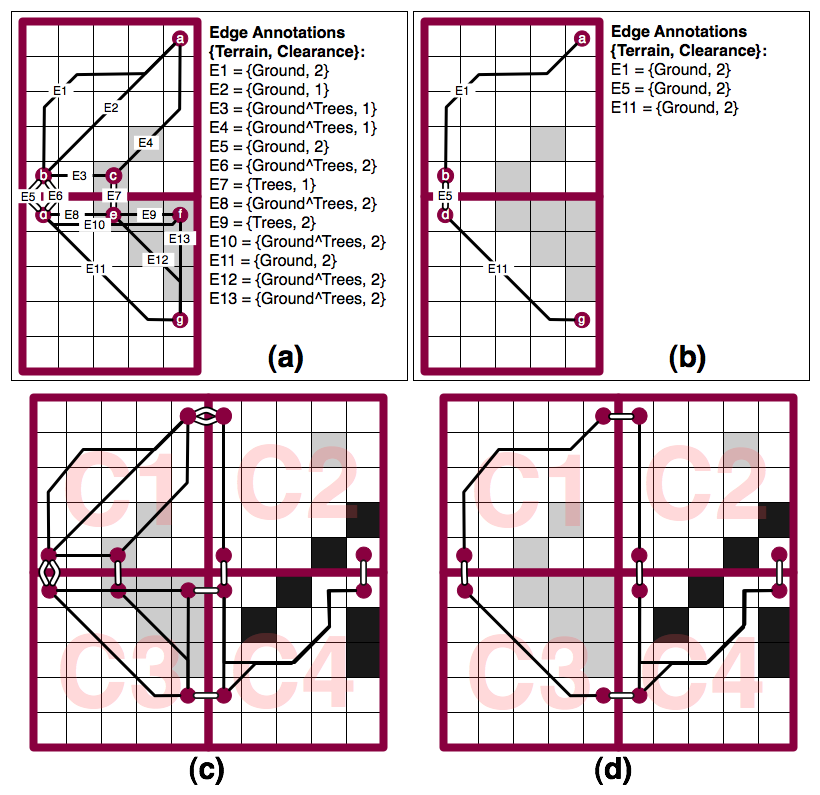
\includegraphics[scale=0.25]{diagrams/clusters_and_entrances.png}
        \end{center}
        \label{aha-fig:abstractgraph}
\end{figure}
